\documentclass[11pt,oneside,openany]{article}

\usepackage{graphicx}
\usepackage{color}    % to define macros for colors
\usepackage{listings} % package to include source code

\author{Matteo Franchin}

\title{Multiphysics~simulations of magnetic~nanostructures}

%TYPESETTING:----------------------------------------------------------

% Reset page margins properly for doublesided pages

% No headings
\pagestyle{plain}

% 1.5 interline spacing --> corresponds to linespread 1.3
% 2.0 interline spacing --> corresponds to linespread 1.6
\linespread{1.3}

\setlength{\marginparwidth}{0mm}
\setlength{\marginparsep}{0mm}
\setlength{\oddsidemargin}{0.7in} % corresponds to 1 + 0.7 = 1.7 inches
\setlength{\evensidemargin}{0.7in} % corresponds to 1.7 inches
\setlength{\textwidth}{145mm}
\setlength{\textheight}{220mm}
\setlength{\voffset}{-20mm}
\raggedbottom

%----------------------------------------------------------------------
% Extra colors

\definecolor{lightgrey}{cmyk}{0.05,0.05,0.05,0}
\definecolor{gray}{rgb}{0.5,0.5,0.5}

%----------------------------------------------------------------------
% Style for code listings

\lstdefinestyle{defaultstyle}{}
\lstset{language=Python}
\lstset{basicstyle=\ttfamily\scriptsize}
\lstset{showstringspaces=false}
\lstset{keywordstyle=\color{blue}}
\lstset{stringstyle=\color{red}}
\lstset{commentstyle=\color{gray}\emph}
\lstset{numbers=left,frame=single}
\lstset{backgroundcolor=\color{lightgrey}}

%----------------------------------------------------------------------
% New commands
\newcommand{\Ms}{M_{\mathrm{sat}}}

\begin{document}

\titlepage

\section{Spatially varying parameters with Nmag5}

\subsection{Introduction}
Sometimes, when studying certain kinds of micromagnetic structures, it is
useful to define material parameters which vary in space. For example, this is
necessary for studying samples with material defects: a defect may be
represented by a localised variation in the saturation magnetisation.  Having
spatially varying parameters is also useful for simulating systems composed by
different materials (e.g. magnetic multilayers).
Unfortunately, this kind of simulations is not possible with the old version of
Nmag, where the material parameters are forced to be constant in space and time
for each \verb|MagMaterial| instance. This limitation is one of the main
reasons for the development of the latest version of the Nmag micromagnetic
software package, Nmag5.

\subsection{The content of this document}
In this document we show how to use Nmag5 to run a simulation where the damping
constant, the gyromagnetic ratio, the saturation magnetisation and the magnetic
anisotropy are varying in space (i.e. are not constant throughout the
material).  We show the source code of a simulation script and explain how it
works.

\subsection{Remarks on the Nmag5 interface}
The previous version of Nmag, Nmag4, did not allow to have spatially varying
material parameters: its user interface was designed without taking this
possibility into account. When developing Nmag5 we then faced a problem: how
can we extend the Nmag interface to allow defining non-homogeneous materials
but keeping --- at the same time --- full compatibility with the old interface?
We want new versions of Nmag to be able to run old scripts, if necessary! The
problem is not solved, yet. Nmag5 currently provides most of the functionality
of Nmag4 (see Section \ref{sec:missing_from_nmag5}) under the same user
interface, but a good interface for the new features of Nmag5 is still to be
found.  The new functionality can be used, but only through quite dirty code.

\subsection{The script}
We want to simulate a bilayer film made by two materials A and B.
We do this by defining one single material, which --- however --- has
material parameters which are piecewise constant in space: each material
parameter has a certain value inside material A and a different value
inside material B. A sketch of the system which is being simulated is
shown in Fig. \ref{fig:sketch}.
\begin{figure}[t]
\begin{center}
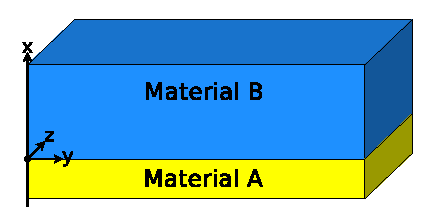
\includegraphics[width=10.0cm]{sketch}
\caption[Sketch]{A sketch of the system simulated in the script.}
\label{fig:sketch}
\end{center}
\end{figure}
The Netgen geo file is shown below:
\lstinputlisting{spatially.geo}

The Nmag script is shown in Fig. \ref{fig:script_1of2} and 
\ref{fig:script_2of2}. A description line-by-line is given below:
\begin{figure}[!p]
\lstinputlisting[linerange=1-46]{spatially.py}
\caption{The first half of the script.}
\label{fig:script_1of2}
\end{figure}

\begin{figure}[!p]
\lstinputlisting[linerange=47-94,firstnumber=47]{spatially.py}
\caption{The second half of the script.}
\label{fig:script_2of2}
\end{figure}

\textbf{Lines 1-9.} The usual Python modules are imported.
Notice that the symbols \verb|Simulation|, \verb|MagMaterial|,
\ldots are imported from \verb|nmag.nmag5| rather than \verb|nmag|.

\textbf{Lines 10-23.} A magnetic material is created similarly to how
it would be done in a normal Nmag script. Here we use dummy material
parameters: we cannot give spatially varying material parameters, as
we are using here the old Nmag4 interface. In other words, the numbers
that appear here are unused (their value is arbitrary), but must be given
in order to comply with the old interface. These parameters will be
redefined later in the script as spatially varying parameters.
Finally, the simulation object is created as usual.

\textbf{Lines 24-26.} These lines are the first Nmag5 specific lines.  We here
specify that the damping constant (\verb|"alpha"|) the saturation magnetisation
(\verb|"Ms"|) the gyromagnetic ratio (\verb|"gamma_G"|) the exchange factor
(\verb|"exchange_factor"|) and the anisotropy constant $K_1$ (\verb|"K1"|) have
to be defined as fields that change continuously in space
(\verb|"spacefield"|). Here there are two things to notice. First, when this
line is not given these quantities are treated as constants, meaning that the
system does not allocate any arrays to store their values. Their values are
inserted directly into the equations of motion and are simplified if possible
(e.g. if \verb|alpha == 0.0|, then the whole damping term is removed).  Second,
the reader must understand here that the quantity \verb|"exchange_factor"| is
not referring to the exchange coupling constant $A$, but rather to the
prefactor of the exchange field $C = 2A/(\mu_0 \Ms)$
($\mathbf{H_{\mathrm{exch}}} = C \, \nabla^2 \mathbf{m}$, where $\mathbf{m} =
\mathbf{M}/\Ms$). This will help to understand some other parts of the script.

\textbf{Lines 27-38.} These lines follow the Nmag4 interfaces.
Briefly: the mesh is loaded, the tolerances for the simulation and
the initial values for the magnetisation and applied field are set.

\textbf{Lines 39-58.} \verb|create_setter| is an helper function which is used
to set the material parameters differently in region A and region B.  We
explain how \verb|create_setter| works with an example.  Imagine you want to
set the initial magnetisation differently in the two layers. Then you need to
pass a function to \verb|Simulation.set_m|. You could do it as follows:
\begin{lstlisting}
m_top = [1, 1, 0]
m_middle = [1, 0, 0]
m_bottom = [1, -1, 0]

def m_setter(r):
  x, y, z = r
  if x < 0.0:
    return m_top
  elif x == 0.0:
    return m_middle
  else: # x > 0.0
    return m_bottom

sim.set_m(m_setter)
\end{lstlisting}
\verb|create_setter| does this for you: it creates and returns a function which
can be used to set a scalar or vector field so that it has different values in
region A, region B and their interface. In particular, the example above may be
rewritten as:
\begin{lstlisting}
m_top = [1, 1, 0]
m_bottom = [1, -1, 0]
m_setter = create_setter(m_bottom, m_top)
sim.set_m(m_setter)
\end{lstlisting}
The \verb|create_setter| function is defined because --- in this script ---
there are many material parameters which have to be set in this way.

\textbf{Lines 59-63.} These lines are useful only for debugging purposes.
Nmag5 does quite a number of ``clever'' things for you: it examines
the equations of motion and understands how one equation may depend on
some others (static dependency inference), it parses the equations
and simplifies the expressions when needed (if there is no spin torque, then
the corresponding term is eliminated from the equations, etc.).
These two lines tell Nmag5 to save to the file \verb|model.desc| information
about what Nmag5 did. These lines can be safely removed from the script
and are there only for debugging purposes.

\textbf{Lines 64-74 and 87-92.} These lines define a dictionary \verb|vs|,
which is used for setting the various spatially inhomogeneous quantities. For
example, the entry
\lstinputlisting[linerange=71-71,firstnumber=71]{spatially.py}
 is used to indicate
that \verb|Ms| (the saturation magnetisation) is measured in units of
\verb|SI("A/m")| and has the value \verb|0.69e6*SI("A/m")| inside the bottom
layer and \verb|0.80e6*SI("A/m")| inside the top layer. This dictionary is
read in the for loop which first extracts the quantity from the
simulation object with \verb|sim.model.quantities[name]| and calls
\verb|create_setter| to set its value. Note that \verb|sim.model| returns
the \verb|Model| object associated to the given simulation object.
See section \ref{sec:nmag5_framework} for details about this.

\textbf{Lines 75-82.} These lines are used to set the exchange factor.
As remarked before, the exchange factor has to be computed from the
exchange coupling constant and the saturation magnetisation through
the formula $C = 2A/(\mu_0 \Ms)$.

\textbf{Lines 83-86.} These lines are used to set the anisotropy constant.
This cannot be done in the for loop, as the quantity must be extracted from
\verb|anisotropy|, rather than from \verb|sim|. This complication is due
to the fact that many anisotropies can be added, and each of them will have
its own constants and its own axes (e.g. \verb|a0_K1| for the first
anisotropy, \verb|a1_K1| for the second, etc.).

\textbf{Lines 93-94.} A relaxation is set up as usual in Nmag4.

\section{What Nmag5 cannot do, yet} \label{sec:missing_from_nmag5}
Here is a list of what is missing from Nmag5:
\begin{itemize}
\item It is not possible to run simulations where the applied field
  changes continuously in time;
\item It cannot simulate 1D and 2D systems (should be easy to fix);
\item Dynamic field dependency is not available, yet. This means that
  if you change the magnetization and probe the demag field, you will
  obtain an out-of-date demag field.
\end{itemize}

\section{The ``nsim.model'' framework} \label{sec:nmag5_framework}
While Nmag4 was built almost directly on top of the special \verb|ocaml| module
(instantiated directly by \verb|pycaml|), Nmag5 is built on top of an
intermediate Python module: \verb|nsim.model|. This module does many of the
things that were done before ``by hand'' (in Nmag4). In particular:
\begin{itemize}
\item it composes the equation of motions for the different materials;
\item it provides an additional layer of abstraction where all the quantities
  appearing inside the equations of motion are used in the same way
  (using the same interface), but are treated in an optimal way when creating
  the simulation model (no memory is allocated for a quantity which is
  declared to be homogeneous in space);
\item does static dependency inference: compute which equation or quantity
  ``is needed'' by which other equation of field;
\item does automatic simplification of equations, alleviating the pain
  of detecing whether a term or matrix should be computed or not.
  For example, if the exchange coupling is set to zero, then the additional
  term is removed from the equation which contains it. This also removes
  the dependency. In other words the exchange matrix is not computed
  when it does not influence the final result.
\end{itemize}

Fig. \ref{fig:nsimmodel} shows how \verb|nsim.model| can be used on its own.
The reader should keep in mind that Nmag5 is built on top of \verb|nsim.model|,
i.e. uses Nmag5 to provide the same interface of Nmag4.
\begin{figure}[!p]
\lstinputlisting{model.py}
\caption{A small example showing nsim.model can be used to simulate
  the Landau-Lifshitz equation.}
\label{fig:nsimmodel}
\end{figure}
%\verb|nsim.model| allows defining equations of motions and quantities that
%appear inside them. If a quantity is constant in time and space, it is
%instantiated with \verb|Constant|, otherwise it is instantiated with
%\verb|SpaceField|.
\end{document}
